\documentclass[11pt,a4paper]{article}
\usepackage[margin=2.2cm]{geometry}
\usepackage[T1]{fontenc}
\usepackage{lmodern,microtype}
\usepackage{graphicx,booktabs,tabularx,float,caption,xcolor,enumitem,amsmath,array,multirow}
\usepackage[hidelinks]{hyperref}
\graphicspath{{../figures/}{../../results/plots/}}
\captionsetup{font=small,labelfont=bf}
\setlist{itemsep=2pt,topsep=4pt}
\newcolumntype{R}{>{\raggedleft\arraybackslash}X}
\makeatletter % float-only pages: stack floats from the top instead of spreading them out
\setlength{\@fptop}{0pt}\setlength{\@fpsep}{14pt}\setlength{\@fpbot}{0pt plus 1fil}
\makeatother

\title{\textbf{Processing and Visualising Large DEMs on a Laptop}\\[4pt]
\large Progress Report, Phase 3: Our Own CPU and GPU Terrain Engine}
\author{Team GeoGuessers \quad|\quad Spatial Informatics\\[4pt]
Swayam Goyal (2024111012) \quad Siddharth Choudhary (2024111021)\\
Yakkala Viswanadha Kartikeya (2024111033)}
\date{}

\begin{document}
\maketitle

\begin{abstract}
\noindent
Phase 2 showed that GDAL's \texttt{gdaldem} never runs out of memory on our laptop but is limited by
single-threaded computation (about 73\% of its run time, 1 of 22 threads used). In Phase 3 we built our own terrain
engine to remove that bottleneck and to find where it moves next. The engine processes a DEM window by window with a
one-cell border (halo) in a three-stage pipeline: parallel reading, a compiled kernel, and one writer thread. It runs
either on the CPU (Numba, all cores) or on the GPU (our own CUDA kernels). It reproduces all ten \texttt{gdaldem}
operator configurations and matches \texttt{gdaldem} on every cell of four full real grids (90\,m to 2\,m). In 985
measured runs on the same grids, harness and machine as Phase 2, the CPU engine computes slope 2.1--3.5$\times$
faster than \texttt{gdaldem} on the same cores (1\,m: 60\,s vs 208\,s) with a flat memory use of about 1.4\,GB,
while a whole-grid NumPy program runs out of memory beyond roughly 0.5--0.7 billion cells. The GPU kernel computes
50$\times$ faster than the CPU kernel, yet the whole run is only 1.0--1.4$\times$ faster (1\,m: 44\,s), because 95\%
of the GPU's own time is copying data and the run is limited by decompressing the input and writing the output.
Computation is no longer the bottleneck: data movement is.
\end{abstract}

\section{Objectives}
The project studies how to process and visualise very large DEMs on one laptop, and where the actual bottleneck
lies (research gap \textbf{G1}: no study reports where standard GDAL/QGIS terrain tools stop being practical,
separated into stages). Phase 2 measured the standard tools. Phase 3 asks:
\begin{enumerate}
  \item How much faster can terrain derivatives be computed when the work is tiled and parallel, on the same
  machine and grids, and with results identical to \texttt{gdaldem}?
  \item Once computation is parallel, which stage limits the run: reading, computing, copying or writing?
  \item When does a GPU actually help, once the cost of copying data to it is counted?
\end{enumerate}

\section{The engine}
\paragraph{Pipeline (CPU).} The grid is processed in $2048\times2048$-cell windows, each read with a one-cell halo so
that the $3\times3$ operators are exact at window edges. Three stages overlap: four reader threads (each with its own
GDAL handle; at most six windows in flight, so memory stays bounded), the compute kernel in the main thread, and a
single writer thread, as GDAL's multi-threading documentation advises against writing from several threads. The
kernel is compiled with Numba \cite{numba} and spread over all cores. Slope, aspect and hillshade can be computed in
one fused pass, since they share the same gradient.

\paragraph{GPU.} The same pipeline with only the compute stage replaced: each window is copied into a pinned
(page-locked) host buffer, copied to the GPU, processed by our own CUDA kernels (compiled at run time through CuPy
\cite{cupy}; one GPU thread per cell, all ten configurations, three products fused), and copied back. Windows
alternate between two CUDA streams, so the copies of one window overlap the kernel of the next. Arithmetic is
float32: GDAL itself adds the Horn neighbour values in float32, and laptop GPUs run float64 far slower.

\paragraph{Operators.} Slope, aspect and hillshade with the Horn \cite{horn} and Zevenbergen--Thorne \cite{zt}
methods, TRI (Riley \cite{riley}, Wilson \cite{wilson}), TPI and roughness, with \texttt{gdaldem}'s conventions
(nodata border, flat-cell aspect, hillshade scaling).

\paragraph{Correctness.} Unit tests (119 in total) compare every kernel with \texttt{gdaldem} on two $1024^2$ crops.
A full-grid check compares the CPU and GPU engines with \texttt{gdaldem} on every cell of the whole 90\,m, 30\,m,
8\,m and 2\,m real grids, for all ten configurations (1.3\,M to 247\,M valid cells per grid). Nodata masks are
identical, and every value is within the test tolerance, with one explained exception. Our float64 CPU engine
differs in Horn aspect on a few nearly flat cells (at most 0.08\% of cells) and in Horn slope on one cell (0.022$^\circ$
against a 0.02$^\circ$ tolerance), because \texttt{gdaldem} adds the Horn neighbours in float32. With that rounding reproduced, every cell matches; the float32 GPU kernel, which adds them
the same way, matches with no exception.

\section{Methodology}
The harness, machine and protocol are those of Phase 2: each run is a separate process, with exact per-process
time, peak memory, CPU and bytes read/written; cold runs empty the Windows file cache first; real grids get 5 cold
and 5 warm runs (plus a warm-up), the synthetic 2\,m and 1\,m grids 3 cold and 1 warm; medians are reported, and
median and IQR of every configuration are kept (median IQR 1.6\% for E3 and 1.2\% for E4). Engine run times include
Python start-up (about 0.5\,s) and loading the compiled kernel, exactly as \texttt{gdaldem}'s times include its
start-up. The machine is an Intel Core Ultra 9 185H (6 performance, 8 efficiency and 2 low-power cores, 22 threads),
16\,GB RAM, NVMe SSD and an NVIDIA RTX 4060 Laptop GPU (8\,GiB).

\paragraph{Experiments.}
\textbf{E3 (CPU engine, 501 runs):} 24 variants on the 8\,m, 2\,m real, 2\,m and 1\,m synthetic grids: all 22
threads or the 12 performance-core threads used by \texttt{gdaldem}; all ten operator configurations; three products
fused; with and without writing; compressed output; 1 to 22 threads; window sizes 512 to 8192; the same pipeline with
a single-threaded NumPy kernel; and a ``naive'' program that reads the whole grid into memory.
\textbf{E4 (GPU engine, 484 runs):} the same grids, the steps of the GPU optimisation (see Section~\ref{sec:ladder}),
float32 vs float64, all operators, fused products, window sizes, and 4 vs 8 reader threads. A separate
\textbf{crossover test} times one window held in memory, from $128^2$ to $8192^2$ cells, on the CPU and the GPU.

\paragraph{GPU safety.} GPU memory use was capped at 4\,GiB. Before every GPU run the harness waited until the GPU
was below 75\,$^\circ$C and it would have stopped the sweep at 85\,$^\circ$C. No clock, power-limit or driver setting
was changed. Over all runs the GPU reached at most 63\,$^\circ$C and used at most 2.0\,GiB.

\section{Results: CPU engine (E3)}
\subsection{Speed and memory}

\begin{table}[!htbp]
\centering\small
\caption{Slope (Horn), engine vs \texttt{gdaldem}, warm cache. ``Same cores'': the engine pinned to the 12
performance-core threads that \texttt{gdaldem} used.}
\label{tab:e3}
\begin{tabularx}{\linewidth}{lrRRRRR}
\toprule
Grid & Cells & \texttt{gdaldem} & Engine, same cores & Speed-up & Engine, 22 threads & Engine peak memory \\
\midrule
8\,m & 169\,M & 4.02\,s & 1.94\,s & 2.1$\times$ & 2.28\,s & 1.35\,GB \\
2\,m real & 264\,M & 6.63\,s & 2.53\,s & 2.6$\times$ & 2.72\,s & 1.37\,GB \\
2\,m synthetic & 2.7\,B & 53.7\,s & 16.3\,s & 3.3$\times$ & 16.4\,s & 1.42\,GB \\
1\,m synthetic & 10.8\,B & 208.4\,s & \textbf{60.3\,s} & \textbf{3.5$\times$} & 68.2\,s & 1.43\,GB \\
\bottomrule
\end{tabularx}
\end{table}

\begin{figure}[!htbp]
\centering
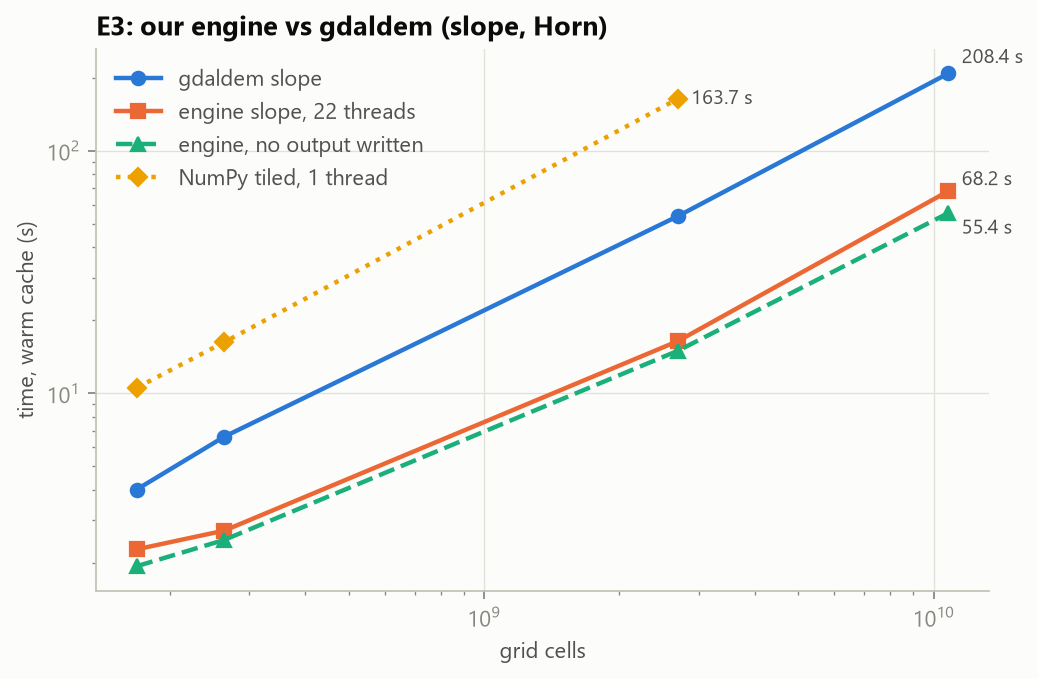
\includegraphics[width=0.49\linewidth]{e3_scaling.png}\hfill
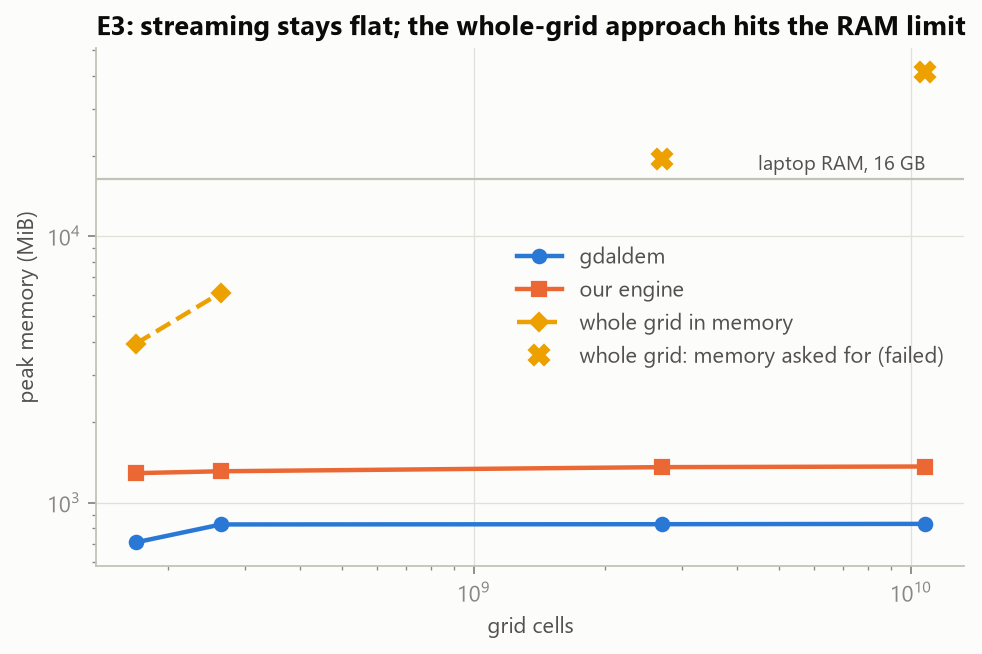
\includegraphics[width=0.49\linewidth]{e3_memory.png}
\caption{Left: run time vs grid size. Right: peak memory. The engine stays flat at about 1.4\,GB; the whole-grid
NumPy program needs about 24 bytes per cell and fails on the 2\,m synthetic and 1\,m grids.}
\label{fig:e3}
\end{figure}

\begin{itemize}
  \item \textbf{2.1--3.5$\times$ faster on the same cores, growing with size.} At 1\,m the engine needs about 5.6\,ns
  per cell against \texttt{gdaldem}'s 19\,ns. Small grids gain less because about 1\,s of every run is fixed cost
  (Python start-up and loading the compiled kernel).
  \item \textbf{12 performance-core threads beat all 22} (1\,m: 60\,s vs 68\,s): the efficiency and low-power
  cores slow the evenly split work down.
  \item \textbf{Memory is flat} at about 1.4\,GB for every size (\texttt{gdaldem}: 0.87\,GB).
  \item \textbf{Where the simple approach breaks.} The naive whole-grid NumPy program needs about 24 bytes per cell
  (4.1\,GB at 8\,m, 6.4\,GB at 2\,m real). On the 2\,m synthetic grid it held 9.6\,GB when a further 10.7\,GB
  allocation was refused (the whole run would need about 65\,GB); at 1\,m its first allocation (43\,GB) was refused.
  On this 16\,GB laptop, whole-grid processing stops working at roughly 0.5--0.7 billion cells; streaming tools
  (\texttt{gdaldem}, our engine) do not have this limit.
  \item \textbf{The speed comes from the compiled parallel kernel, not from tiling alone}: the same pipeline with a
  single-threaded NumPy kernel is 2.6--3$\times$ \emph{slower} than \texttt{gdaldem}.
\end{itemize}

\subsection{Every operator, and three products in one pass}
All ten \texttt{gdaldem} configurations run 1.3--2.0$\times$ faster at 8\,m and 1.7--2.6$\times$ faster on the
2\,m real grid (Figure~\ref{fig:ops}). On these grids the engine takes the same time for every operator (2.0--2.3\,s
and 2.4--2.8\,s): fixed start-up and I/O dominate, not the arithmetic. The gain is largest for slope and aspect,
\texttt{gdaldem}'s most expensive operators (23--27\,ns per cell).

\begin{figure}[!htbp]
\centering
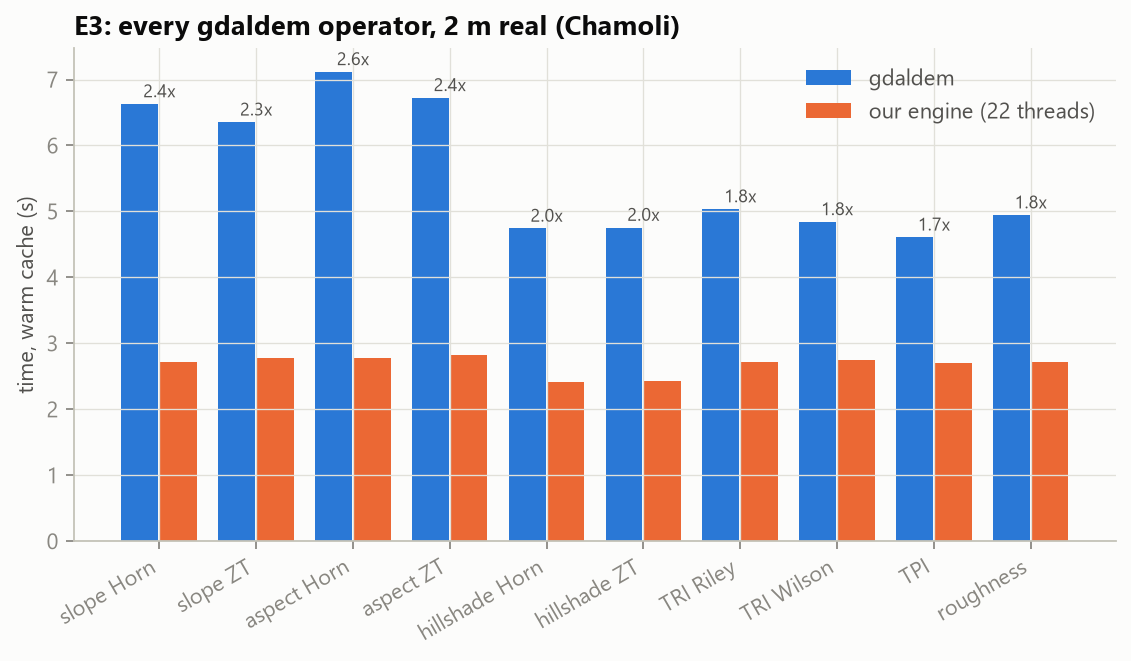
\includegraphics[width=0.49\linewidth]{e3_operators.png}\hfill
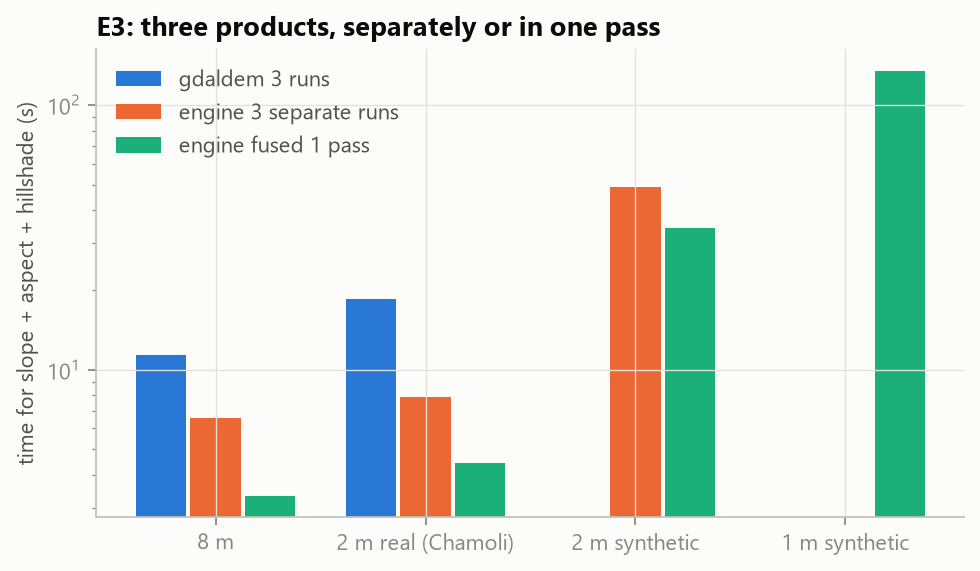
\includegraphics[width=0.49\linewidth]{e3_products.png}
\caption{Left: all ten configurations on the 2\,m real grid. Right: slope + aspect + hillshade as three separate
runs or one fused pass.}
\label{fig:ops}
\end{figure}

\begin{table}[!htbp]
\centering\small
\caption{Slope + aspect + hillshade, warm cache. \texttt{gdaldem} was not run for aspect on the synthetic grids,
so only slope + hillshade can be compared there (a lower bound for the gain).}
\begin{tabularx}{\linewidth}{lRRRR}
\toprule
Grid & \texttt{gdaldem}, 3 runs & Engine, 3 runs & Engine, one fused pass & Fused vs \texttt{gdaldem} \\
\midrule
8\,m & 11.3\,s & 6.6\,s & \textbf{3.3\,s} & 3.4$\times$ \\
2\,m real & 18.5\,s & 7.9\,s & \textbf{4.4\,s} & 4.2$\times$ \\
2\,m synthetic & ($>$94.7\,s) & 49.0\,s & \textbf{34.4\,s} & $\geq$2.8$\times$ \\
1\,m synthetic & ($>$367\,s) & -- & \textbf{134.8\,s} & $\geq$2.7$\times$ \\
\bottomrule
\end{tabularx}
\end{table}

\subsection{Where the engine's time goes}

\begin{table}[!htbp]
\centering\small
\caption{Slope, all 22 threads, warm cache. ``Wait'' columns: time the compute thread sat idle; the writer thread
works in parallel, ``writer busy'' is its own working time.}
\label{tab:stages}
\begin{tabularx}{\linewidth}{lRRRRRRR}
\toprule
Grid & Total & Start-up & Wait for input & Compute & Wait for writer & Writer busy & Written \\
\midrule
8\,m & 2.28\,s & 0.52\,s & 0.27\,s & 0.98\,s & 0.25\,s & 1.01\,s & 0.71\,GB \\
2\,m real & 2.72\,s & 0.50\,s & 0.39\,s & 1.24\,s & 0.30\,s & 1.48\,s & 1.10\,GB \\
2\,m synthetic & 16.4\,s & 0.63\,s & 3.4\,s & 8.9\,s & 3.3\,s & 14.6\,s & 10.9\,GB \\
1\,m synthetic & 68.2\,s & 0.62\,s & 9.3\,s & 33.1\,s & 24.8\,s & \textbf{65.3\,s} & 43.4\,GB \\
1\,m, no output & 55.4\,s & 0.60\,s & \textbf{22.9\,s} & 31.4\,s & 0 & 0 & 0 \\
\bottomrule
\end{tabularx}
\end{table}

\begin{itemize}
  \item \textbf{The run is now limited by moving data.} At 1\,m the kernel needs 33\,s, while the single writer
  thread is busy for 65\,s writing 43\,GB (about 0.66\,GB/s): the run is \emph{write-bound}. Without writing it is
  \emph{read-bound}: 23\,s waiting for windows to be decompressed.
  \item \textbf{Reading is limited by decompression, not by the disk.} With no output, 8 reader threads instead of 4
  cut the read wait on the 2\,m synthetic grid from 5.8\,s to 1.2\,s; with output written the change gives nothing,
  because the writer is then the limit. Cold vs warm cache changes almost nothing (1\,m: 67\,s vs 68\,s).
  \item \textbf{Compressed output} (ZSTD level 1) is 40\% smaller (6.6\,GB vs 10.9\,GB at 2\,m synthetic) but slower
  (21.2\,s vs 16.4\,s), since compression takes CPU away from the kernel.
\end{itemize}

\subsection{Threads and window size}

\begin{figure}[!htbp]
\centering
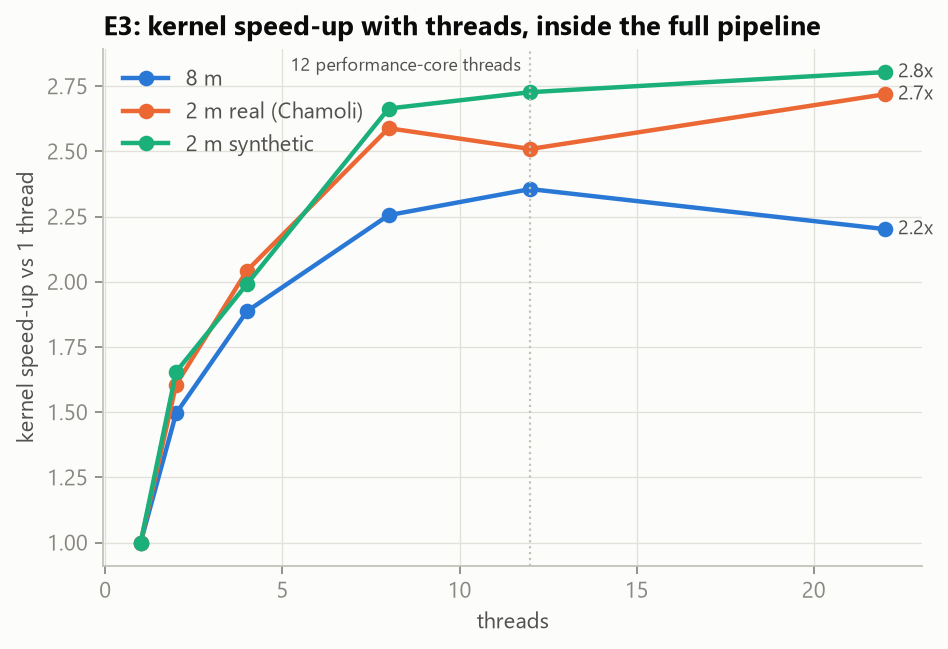
\includegraphics[width=0.45\linewidth]{e3_threads.png}\hfill
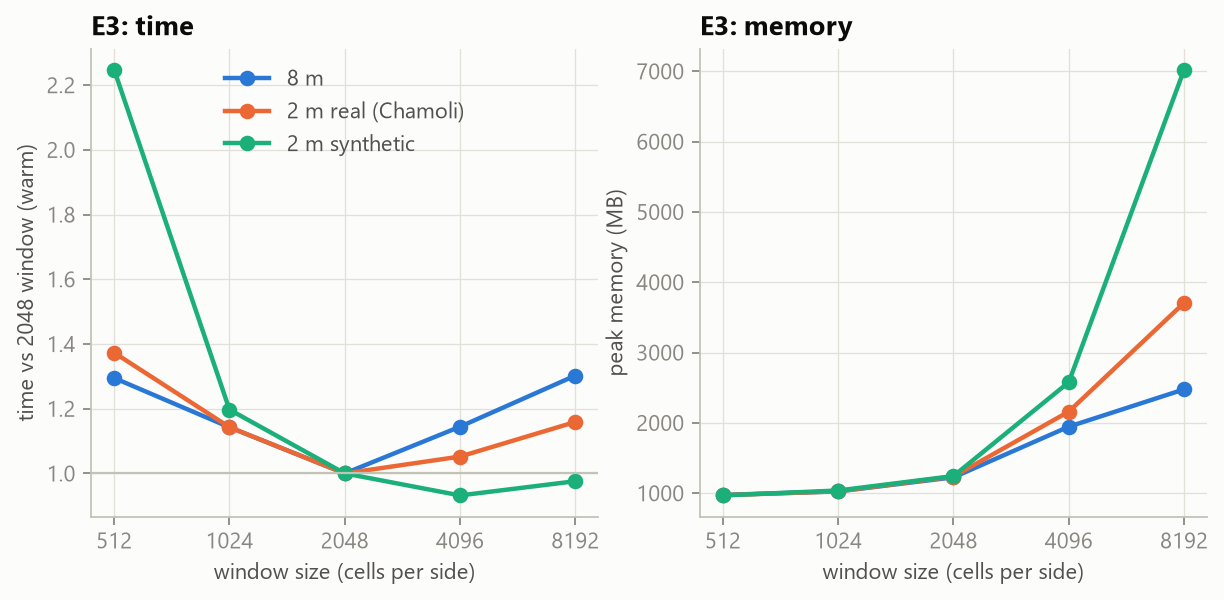
\includegraphics[width=0.53\linewidth]{e3_window.png}
\caption{Left: kernel speed-up with threads inside the full pipeline. Right: run time (relative to the default 2048
window) and peak memory for window sizes 512--8192.}
\label{fig:threads}
\end{figure}

\begin{itemize}
  \item \textbf{More threads stop helping early.} Inside the pipeline the kernel speeds up only 2.2--2.8$\times$
  from 1 to 22 threads; on its own, in memory, it scales to about 16 threads (9.5\,ns per cell with 1 thread,
  1.7\,ns with 16). In the pipeline it shares the cores with decompression and writing, and the slower efficiency
  cores hold the other threads up. Beyond 4--8 threads the total time hardly changes.
  \item \textbf{2048$\times$2048 windows are the best size.} Small windows are slow because of the halo: the input is
  stored in compressed $512\times512$ tiles, and each window's one-cell border forces the neighbouring tiles to be
  decompressed again, $(w/512+2)^2$ tiles instead of $(w/512)^2$, i.e.\ 9$\times$ extra work at $w=512$ and
  2.25$\times$ at 2048. A 512 window is up to 2.2$\times$ slower; an 8192 window holds 7.4\,GB in flight for no gain.
\end{itemize}

\section{Results: GPU engine (E4)}
\subsection{Speed}

\begin{table}[!htbp]
\centering\small
\caption{Slope (Horn), warm cache: \texttt{gdaldem}, CPU engine (12 threads) and GPU engine.}
\label{tab:e4}
\begin{tabularx}{\linewidth}{lRRRRRR}
\toprule
Grid & \texttt{gdaldem} & CPU engine & GPU engine & GPU vs CPU & GPU vs \texttt{gdaldem} & GPU, no output \\
\midrule
8\,m & 4.02\,s & 1.94\,s & 1.90\,s & 1.0$\times$ & 2.1$\times$ & 1.80\,s \\
2\,m real & 6.63\,s & 2.53\,s & 2.18\,s & 1.2$\times$ & 3.0$\times$ & 2.03\,s \\
2\,m synthetic & 53.7\,s & 16.3\,s & \textbf{11.3\,s} & 1.4$\times$ & 4.7$\times$ & 9.3\,s \\
1\,m synthetic & 208.4\,s & 60.3\,s & \textbf{43.8\,s} & 1.4$\times$ & \textbf{4.75$\times$} & 33.9\,s \\
\bottomrule
\end{tabularx}
\end{table}

\begin{figure}[!htbp]
\centering
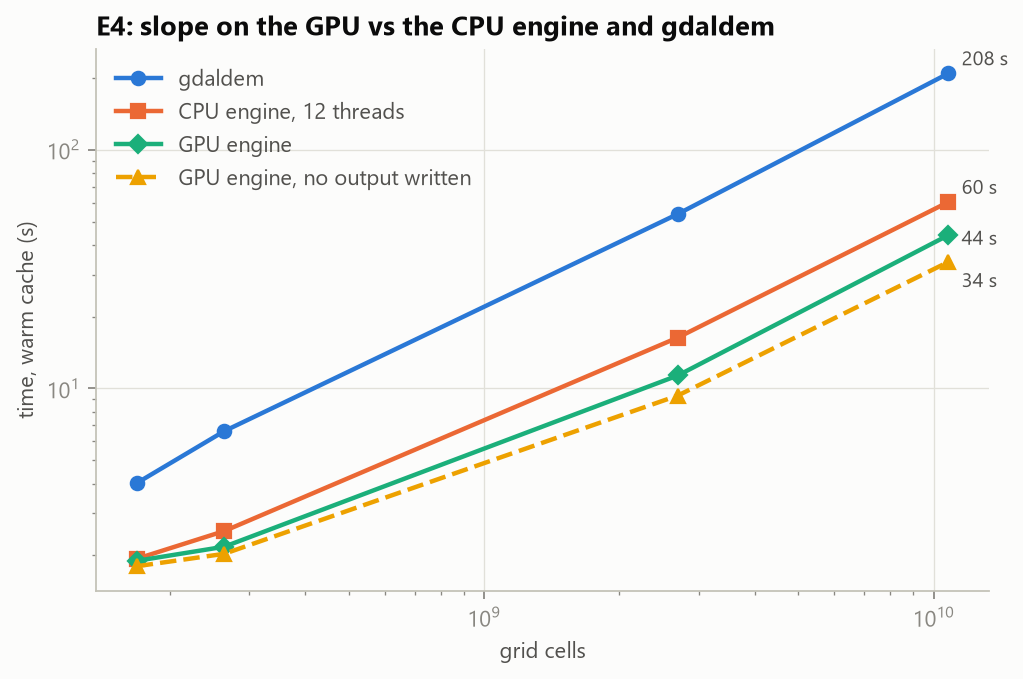
\includegraphics[width=0.49\linewidth]{e4_scaling.png}\hfill
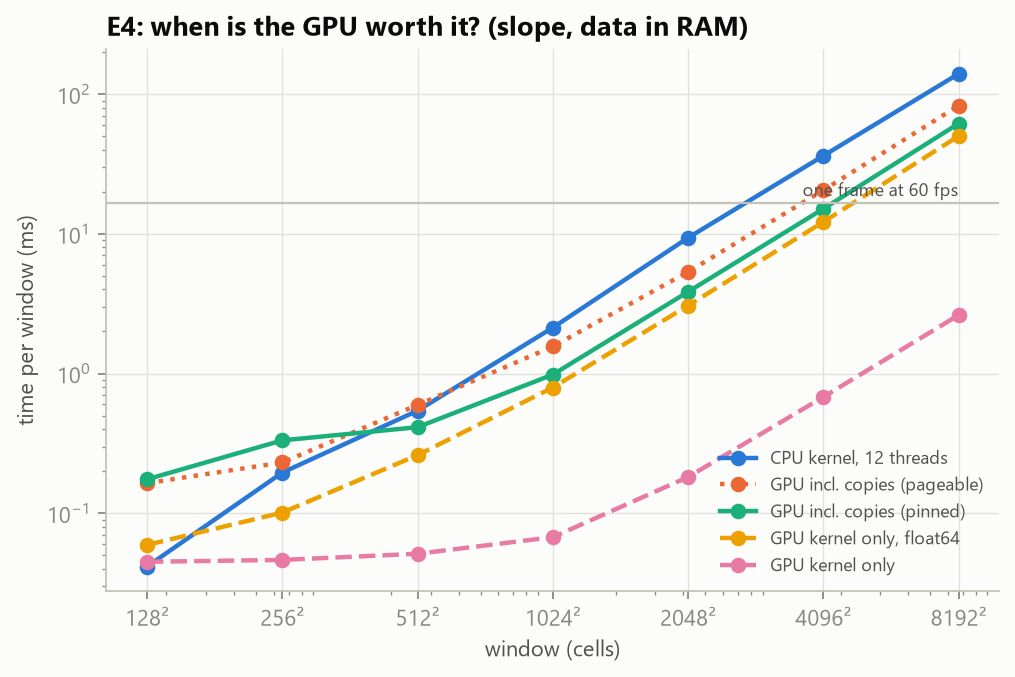
\includegraphics[width=0.49\linewidth]{e4_crossover.png}
\caption{Left: slope run time vs grid size. Right: one window held in memory: the GPU kernel alone is about
50$\times$ faster than the 12-thread CPU kernel, but with the copies it is only 2.2--2.4$\times$ faster, and below
about $512^2$ cells it is slower than the CPU.}
\label{fig:e4}
\end{figure}

\begin{itemize}
  \item \textbf{The GPU computes 50$\times$ faster, but the run is only 1.0--1.4$\times$ faster.} The GPU kernel
  needs 1.1\,s for the whole 10.8-billion-cell grid, where the CPU engine's kernel needed 34\,s.
  \item \textbf{Copying is 95\% of the GPU's own time.} For a $2048^2$ window the kernel takes 0.18\,ms and kernel
  plus copies 3.85\,ms. Crossing PCIe, not computing, is the GPU's cost.
  \item \textbf{The GPU only pays off above a minimum size}: from $512^2$ cells for slope and $256^2$ for three
  products. Below, a GPU round trip (at least $\sim$0.17\,ms) is slower than the CPU kernel.
  \item \textbf{Three products gain the most}: one fused pass takes 81\,s at 1\,m vs 135\,s on the CPU (1.7$\times$),
  and 3.1\,s on the 2\,m real grid vs 18.5\,s for three \texttt{gdaldem} runs (5.9$\times$).
  \item \textbf{GPU memory is never the limit}: window by window the engine uses at most 2.0\,GiB of the 8\,GiB.
  Sending a whole grid at once would need 22\,GB at 2\,m synthetic and 86\,GB at 1\,m; as on the CPU, only
  tiling scales.
\end{itemize}

\subsection{The bottleneck moves}

\begin{figure}[!htbp]
\centering
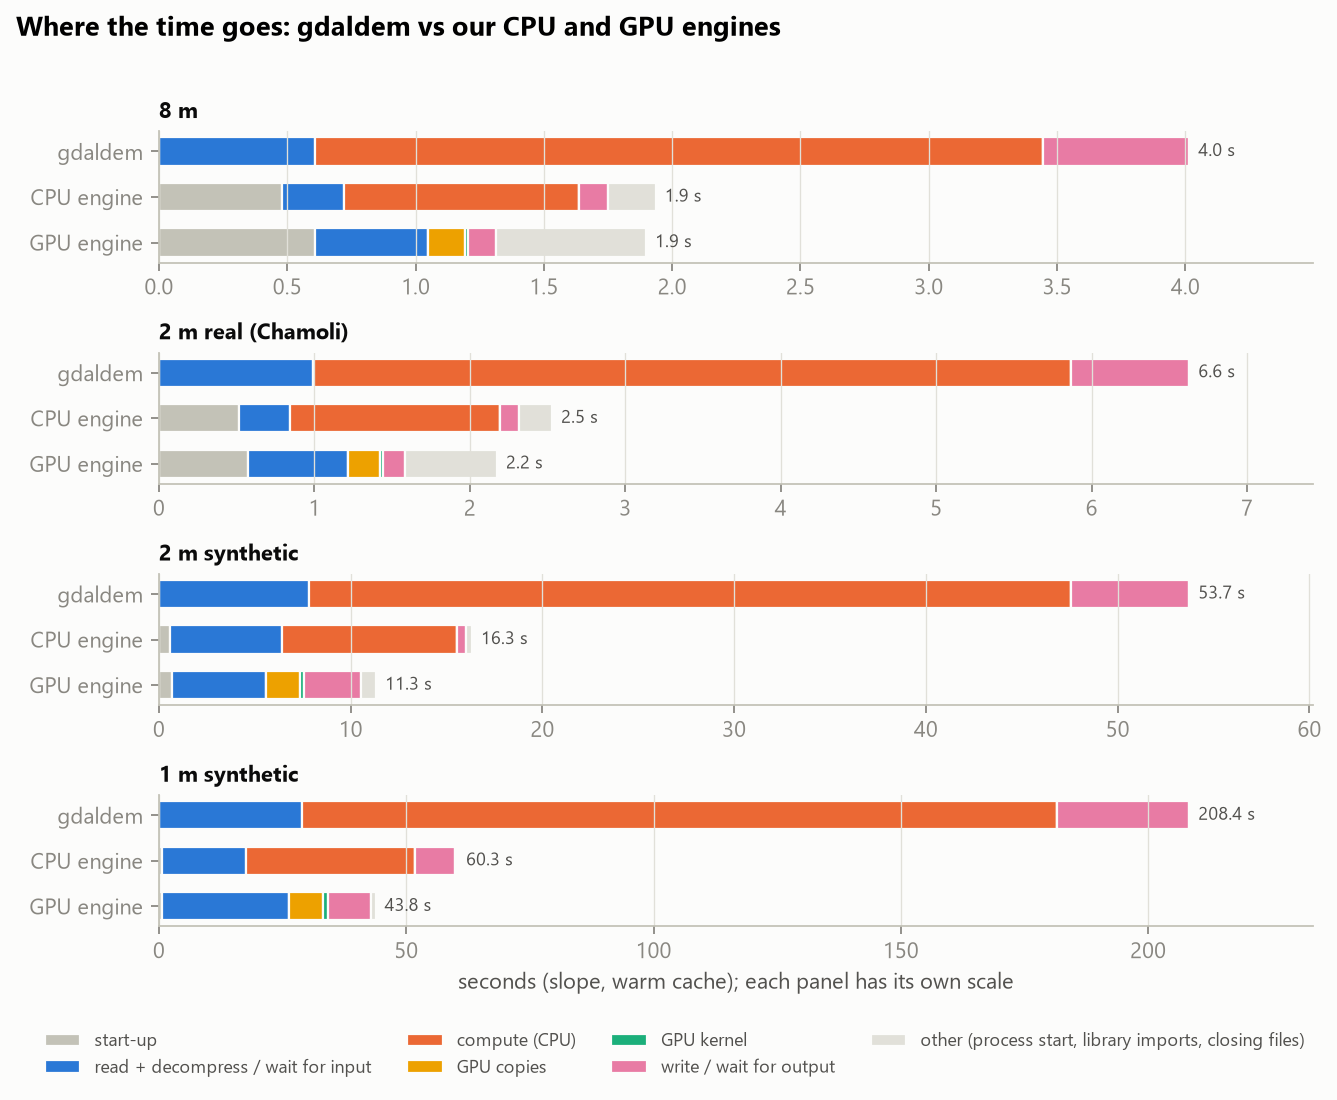
\includegraphics[width=0.86\linewidth]{e4_stages.png}
\caption{Where the time goes (slope, warm). \texttt{gdaldem}: stages from the Phase 2 stage split, one after the
other. Engines: how the main thread spends the run (the writer works in parallel, so only waiting for it appears).
From \texttt{gdaldem} to the CPU engine to the GPU engine, computation (orange, green) shrinks and reading, copying
and writing remain.}
\label{fig:stages}
\end{figure}

At 1\,m the GPU engine's main thread spends 25.7\,s waiting for input to be decompressed and only 7.8\,s on the GPU.
With 8 reader threads instead of 4 the read wait falls to 3.2\,s, but the writer then becomes the limit (wait 30.6\,s
for 43\,GB at about 1.1\,GB/s) and the total only goes from 43.8\,s to 42.6\,s. Each fix exposes the next stage:
\emph{computation $\rightarrow$ decompression $\rightarrow$ writing}.

\subsection{How the GPU is used matters more than the GPU}
\label{sec:ladder}

\begin{figure}[!htbp]
\centering
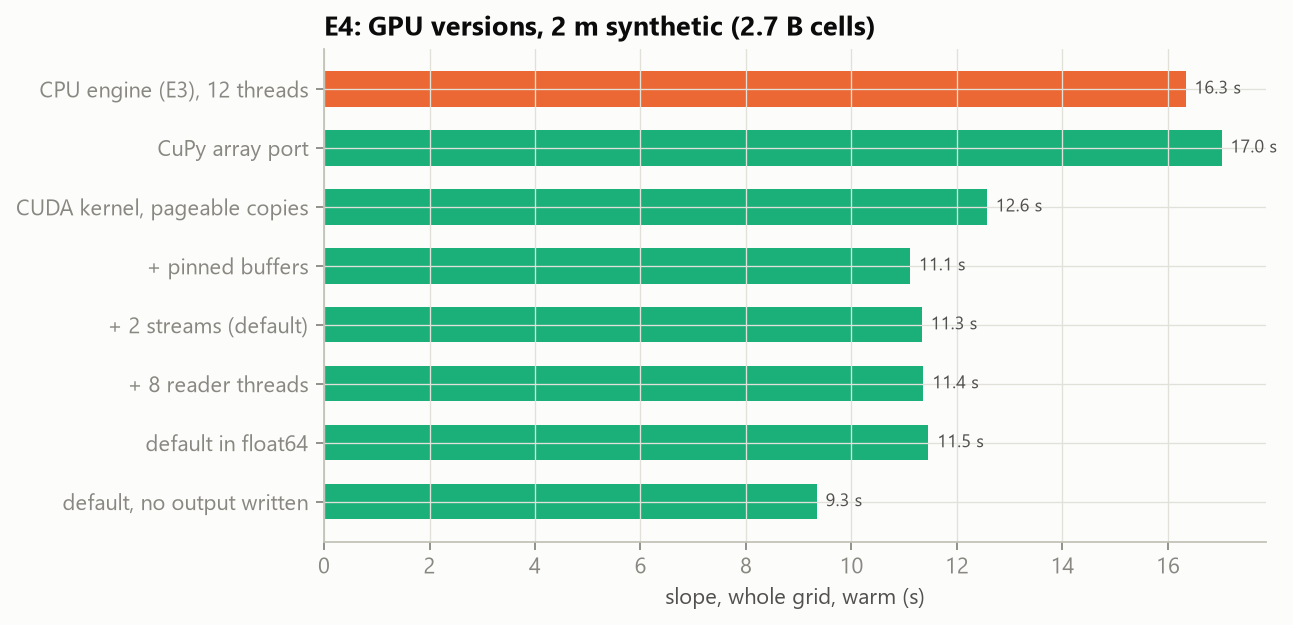
\includegraphics[width=0.72\linewidth]{e4_ladder.png}
\caption{Slope on the 2\,m synthetic grid (2.7 billion cells), warm: the steps from a straightforward GPU port to
our default GPU engine, against the CPU engine.}
\label{fig:ladder}
\end{figure}

The straightforward port (the NumPy code run through CuPy arrays, float64, a temporary array for every intermediate
result) takes 17.0\,s, \emph{slower} than the CPU engine (16.3\,s). Our own CUDA kernel brings it to 12.6\,s, pinned
buffers to 11.1\,s. Each step roughly halves the GPU stage (14.5 $\rightarrow$ 7.6 $\rightarrow$ 3.7 $\rightarrow$
2.0\,s with two streams), but the total stops improving once reading and writing dominate. float64 arithmetic makes
the kernel 8--24$\times$ slower and changes the total by almost nothing (11.5\,s vs 11.3\,s); float32 already matches
\texttt{gdaldem}'s Horn rounding, so it is the default.

\section{Discussion}
\paragraph{Where the bottleneck is (G1).} On this laptop the limiting stage depends on the tool:
\texttt{gdaldem} is limited by single-threaded computation; our parallel CPU engine removes most of it and becomes
limited by decompressing the input and writing the output; the GPU removes computation almost entirely, and what is
left is reading, writing and copying over PCIe. A GPU is worth adding where computation is still a large share:
several products at once, heavier operators, or results that are not written to disk.

\paragraph{Implications for the next phases.} For batch processing of whole grids, the next gains must come from I/O
(not writing full-resolution products, compressing them with spare cores, or a faster disk), not from faster
kernels. For on-demand display (Phases 4--5) computation is cheap on both devices: a $512^2$ tile takes 0.5\,ms
(slope) or 1.3\,ms (three products) on the CPU and 0.4--0.5\,ms on the GPU including copies. The time per view will
be set by reading and decoding the elevation data, which the pyramid and a cache of decoded data address. Because a
window's halo touches up to nine stored tiles, the viewer's server should cache decoded data.

\paragraph{Validity.} 985 runs, with two failures, both the intended out-of-memory runs of the naive program.
Medians are reported; the median IQR is 1.6\% (E3) and 1.2\% (E4) of the median. On the 1\,m grid warm values are
single runs. A few numbers (kernel scaling in memory, reader-thread checks) come from one-off in-process tests and
are labelled as such in the project documentation. Sizes use MB = $10^6$ and GB = $10^9$ bytes; GPU memory is in GiB.

\section{Next steps}
\begin{enumerate}
  \item \textbf{Pyramid on demand (E5, gap G2):} compute slope and aspect directly from each pyramid level and
  measure the error against the real 2\,m data, together with the time saved (Phase 4, completed separately).
  \item \textbf{Box-zoom viewer (E6):} the whole map is shown first; the user drags a box on it, and only that box
  is computed, at the pyramid level where one cell is about one screen pixel (or exactly from full resolution on
  request). Nested boxes zoom deeper, down to full resolution. A web viewer and a QGIS plugin share one server; we
  will measure the time per zoom step by stage, CPU vs GPU, at every zoom depth.
\end{enumerate}

\begin{thebibliography}{9}\small
\bibitem{numba} Lam, S.\,K., Pitrou, A., \& Seibert, S. (2015). Numba: A LLVM-based Python JIT compiler.
\emph{Proc.\ Second Workshop on the LLVM Compiler Infrastructure in HPC}, 1--6.
\bibitem{cupy} Okuta, R., Unno, Y., Nishino, D., Hido, S., \& Loomis, C. (2017). CuPy: A NumPy-compatible library
for NVIDIA GPU calculations. \emph{Workshop on Machine Learning Systems (LearningSys), NIPS 2017}.
\bibitem{horn} Horn, B.\,K.\,P. (1981). Hill shading and the reflectance map. \emph{Proceedings of the IEEE},
69(1), 14--47.
\bibitem{zt} Zevenbergen, L.\,W., \& Thorne, C.\,R. (1987). Quantitative analysis of land surface topography.
\emph{Earth Surface Processes and Landforms}, 12(1), 47--56.
\bibitem{riley} Riley, S.\,J., DeGloria, S.\,D., \& Elliot, R. (1999). A terrain ruggedness index that quantifies
topographic heterogeneity. \emph{Intermountain Journal of Sciences}, 5(1--4), 23--27.
\bibitem{wilson} Wilson, M.\,F.\,J., O'Connell, B., Brown, C., Guinan, J.\,C., \& Grehan, A.\,J. (2007).
Multiscale terrain analysis of multibeam bathymetry data for habitat mapping on the continental slope.
\emph{Marine Geodesy}, 30(1--2), 3--35.
\end{thebibliography}

\end{document}
